% Report skeleton — headings, figure slots and table slots only. All prose is yours to write.
% Copy to report_draft.tex, fill in, then run:  python -m experiments.originality_check report_kit/report_draft.tex
\documentclass[12pt,a4paper]{article}
\usepackage[margin=2.5cm]{geometry}
\usepackage{graphicx,booktabs,longtable,hyperref,float}
\graphicspath{{../reports/study/figures/}}
\title{TITLE OF YOUR PROJECT}
\author{NAMES, REGISTRATION NUMBERS \\ GUIDE, DEPARTMENT, UNIVERSITY}
\date{\today}

\begin{document}
\maketitle

\begin{abstract}
% 150--200 words: problem, what was built, data, headline numbers (from fact_sheet.md), one limitation.
\end{abstract}

\section{Introduction}
% Problem, why explanations matter, gap, objectives, outline. Cite what you have read.

\section{Related Work and Comparison}
% Short narrative, then the comparison table (see comparison_table.md; verify every cell).

\section{Proposed Framework}
% Explain the diagram in your words, then the numbered procedural steps.
\begin{figure}[H]\centering
  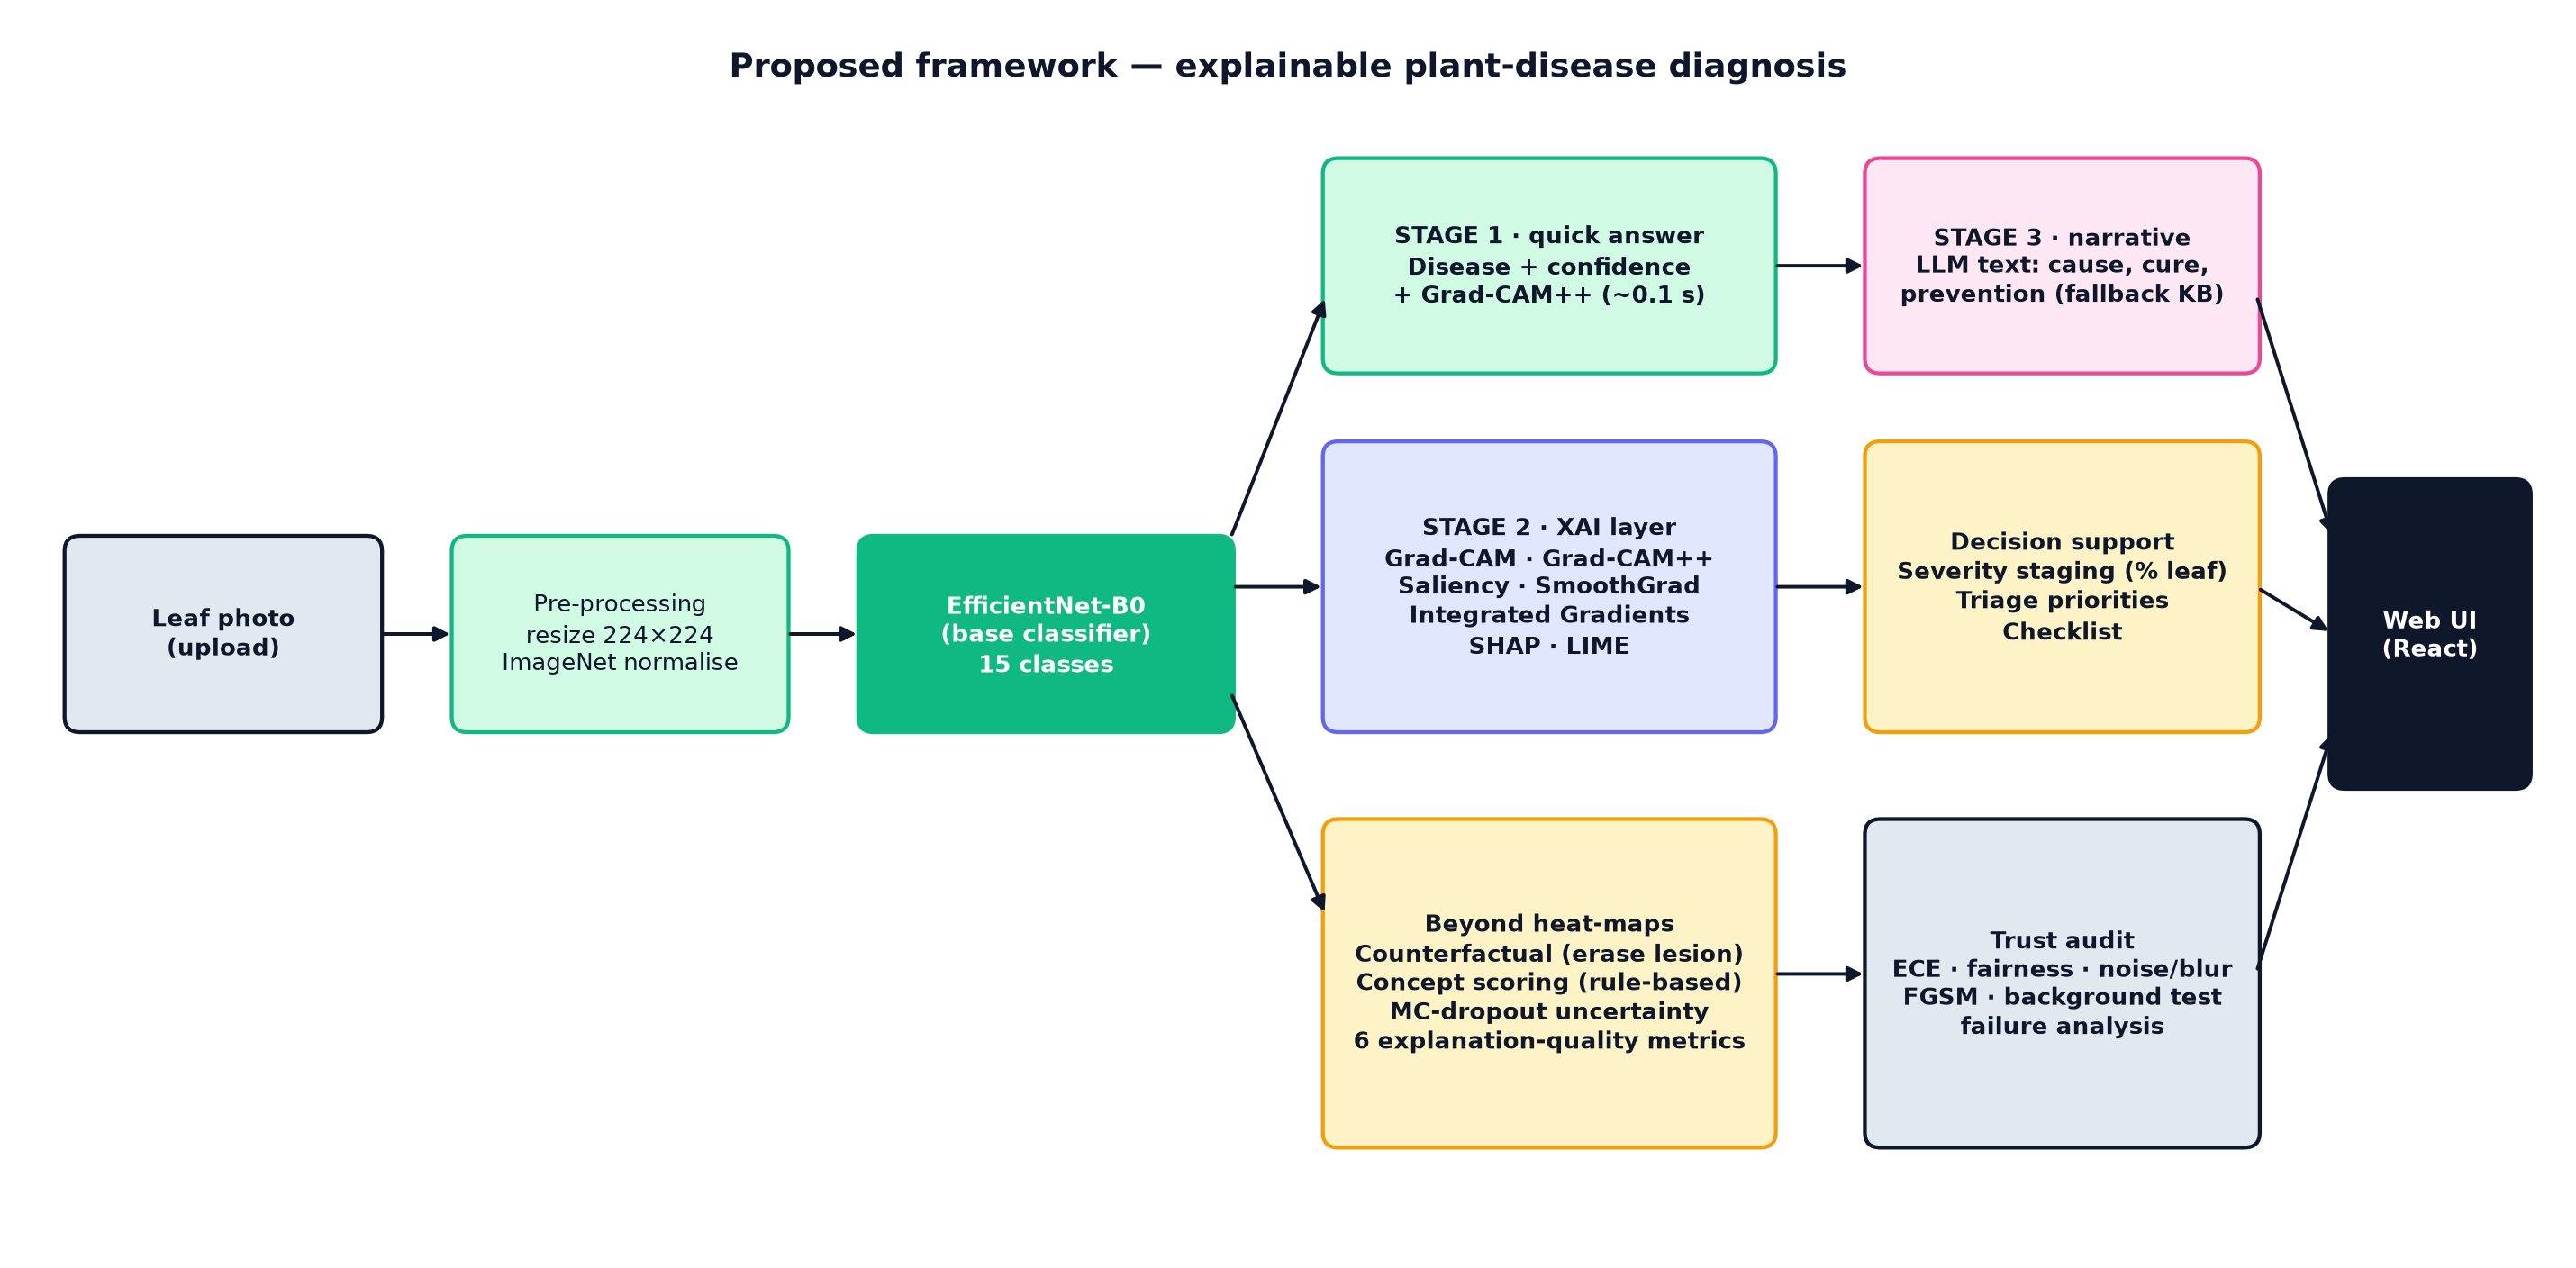
\includegraphics[width=\textwidth]{fig_architecture_system.png}
  \caption{CAPTION}\label{fig:arch}
\end{figure}
\begin{figure}[H]\centering
  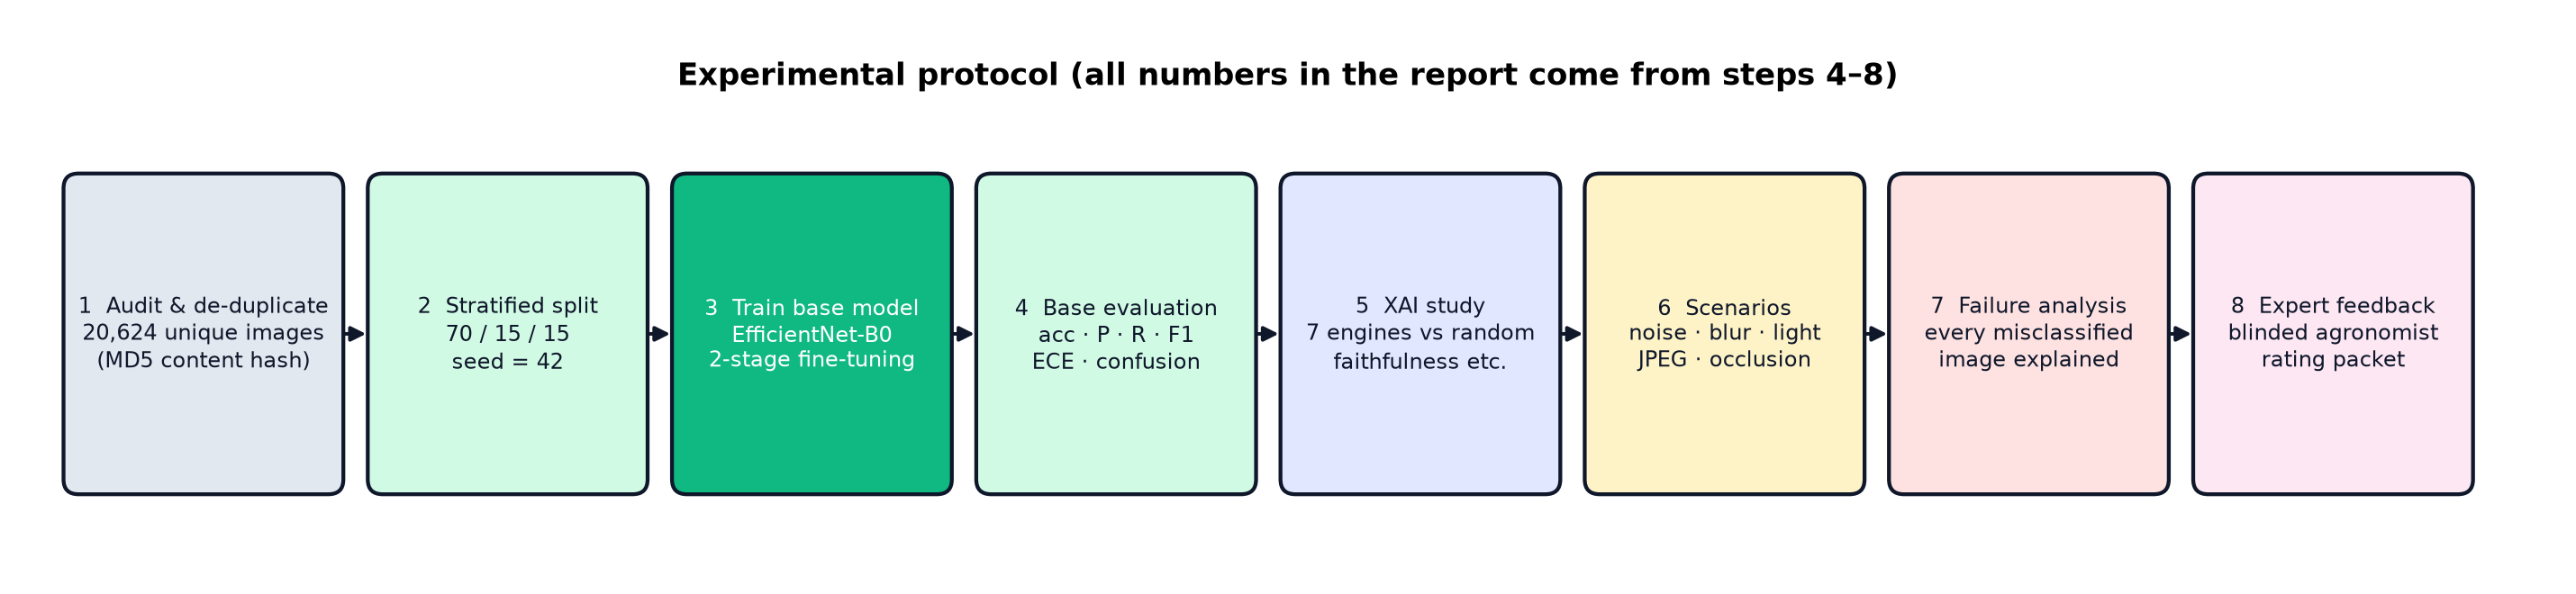
\includegraphics[width=\textwidth]{fig_architecture_protocol.png}
  \caption{CAPTION}\label{fig:protocol}
\end{figure}

\section{Dataset}
% Source, classes, counts before/after deduplication, split, leakage finding.
% Table: reports/study/table_dataset.md   Figures: fig_dataset_distribution.png, fig_dataset_samples.png

\section{Experimental Setup}
% Hardware, software versions, training schedule, evaluation protocols.

\section{Results: Base Model}
% Metrics table, curves, confusion matrix, calibration, error detection. No XAI in this section.

\section{Results: Model with Explainability}
\subsection{Scenario A: clean images, all methods}
\subsection{Scenario B: input perturbations}
\subsection{Scenario C: correct versus wrong predictions}
\subsection{Agreement between methods and runtime}

\section{Analysis with Respect to Features and Metrics}

\section{Human Expert Feedback}
% State who rated, how many cases, protocol, results. If pending: say so.

\section{Failure Cases}

\section{Novel Contributions}
\begin{enumerate}
% one item per contribution; see novel_contributions.md
\end{enumerate}

\section{Limitations}

\section{Conclusion and Future Work}

\bibliographystyle{ieeetr}
\bibliography{references}
\end{document}
